
\chapter{Single top quark production with a photon in the Standard Model}
\label{chap:tqgamma_production}
\section{A brief overview of the Standard Model}

The Standard Model (SM) of particle physics, a quantum field theory,  describes today's best knowledge of elementary physics. 
In the SM, there are different kinds of elementary particles and three fundamental forces of nature: the electromagnetic force, the strong force and the weak force. 
Every force coincides with an elementary particle, called a boson that acts as a mediator of the interaction. Another group of particles are called the fermions and they only interact with these bosons if they have specific quantities, which are represented by their quantum numbers.

The fermions have spin $s = \frac{1}{2}$ and can be divided into two separate groups. The first group, named quarks, are colour charge carrying fermions. 
There are three up-type quarks (up, strange and top) with an electric charge of $q = +\frac{2}{3}e$ and three down-type quarks (down, charm and bottom) with an electric charge of $q = -\frac{1}{3}e$. 
The second group are the leptons. Three leptons (electron, muon and tau) have an electric charge of $q = +1e$. Furthermore, each of these leptons has a corresponding uncharged lepton partner called a neutrino.
Three different families further categorize leptons and quarks. These quark and lepton families are ordered by mass and consist of an up-type quark, the corresponding down-type quark, a lepton and the corresponding neutrino. 
There is an anti-matter particle equivalent for all fermions where every charge-like quantum number has the opposite sign. 

Particles with integer spin are called bosons. The SM lists four different bosons, called gauge bosons, with spin $s = 1$: $gluons$, $photons$, $Z$ and $W^{\pm}$. The Higgs boson is the only boson with spin $s=0$.
Gluons are colour charged and mediate the strong force. They only couple to colour charged particles, including themselves. Photons mediate the electromagnetic (EM) between electrically charged particles. The massive bosons, $Z$ and $W^{-}$ as well as $W^{+}$ mediate the weak force. They couple to particles with weak isospin. Additionally, the $W^{\pm}$ bosons is electrically charged, $q = \pm 1e$, and changes the flavour of a quark when coupling to it.
The Higgs boson explains how particles have mass. The boson arises from the electroweak theory and gives mass to particles via the Higgs mechanism. 

An overview of the elementary particles in the Standard Model is given in figure \ref{fig:standard_model}.

\begin{figure}
    \centering
    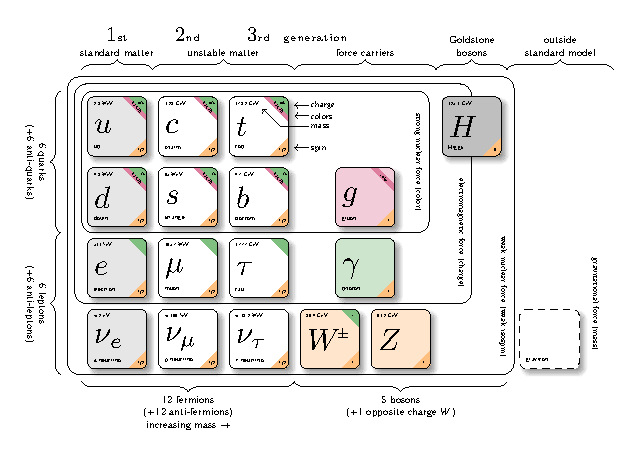
\includegraphics[width=0.9\textwidth]{Plots/model-physics.pdf}
    \caption{Elementary particles of the Standard Model alongside their properties \cite{sm_table}.}
    \label{fig:standard_model}
\end{figure}

\section{The \texorpdfstring{$tq\gamma$}{tqGamma} process in the Standard Model}


The top quark is an up-type quark and the most massive quark of the Standard Model with a mass of $m_t = 173.76 \pm 0.3 \,\si{\giga\electronvolt} (S =1.2)$ \cite{pdg}. Additionally, the top quark has a very small decay width of $\Gamma = 1.42^{+0.19}_{-0.15} \,\si{\giga\electronvolt} (S=1.4)$ \cite{pdg} because of its high mass.
For this reason, top quarks cannot build any bound states and always decay shortly after production. Top quarks are therefore never observed directly. Instead, only their decay products are observable and can be retraced back to the top quark. 

The top quark was first discovered in pair production at the Tevatron in 1995 during a proton-antiproton collision experiment (CITE). In 2009, the D0 \cite{singletop1} and CDF \cite{singletop2} collaborations also separately confirmed the observation of the single-top-quark-process (tq) of the Standard Model at the Tevatron. The combined results are available in Ref. \cite{singletop3}. 
The CMS experiment at the Large Hadron Collider (LHC) of CERN \cite{CMS} reported evidence for the single-top-quark-process with an additional photon ($tq\gamma$) with a significance corresponding to $\sigma = 4.4$. The fiducial cross section 
was measured to be $\sigma(pp\rightarrow tq\gamma)(t\rightarrow\mu \nu b) = 115 \pm 17 (stat) \pm 30 (syst) \,\si{\femto\barn}$ for the photon transverse momentum $p_T^\gamma > 25 \,\si{\giga\electronvolt}$ (CITE). 

For this thesis, the $tq\gamma$-events are produced in proton-proton-collisoins inside the ATLAS experiment. The ATLAS is discussed in detail in chapter \ref{chap:measurement}. The production of processes in this experiment occurs with elementary particles inside of the protons, called partons. For the production of the $tq\gamma$-process, one gluon provided by the protons may produce a bottom-antibottom-quark pair. The bottom quark may then exchange a $W$-boson with a quark, turning the bottom quark into a top quark and changing the flavour of the quark. This top quark may then radiate a photon. 
It is essential to mention that while this thesis focuses on the top-photon vertex, the photon can be radiated from any charged particle elsewhere in the process. For instance, the bottom quark after the decay of the top may produce a photon.
The decay mode of the top quark follows this process. Top quarks decay by emitting a $W^+$-boson and turning into a bottom quark. The $W^+$-boson then decays either into an antilepton and neutrino pair or a quark-antiquark pair of opposite quark types. However, only the leptonic decay mode is considered in this thesis.

In Figure \ref{fig:feyn_tqGamma} the leading order Feynman diagram for the $tq\gamma$ production is depicted. The charge conjugated diagram is not shown, but also considered in this thesis.
\begin{figure}
    \centering
    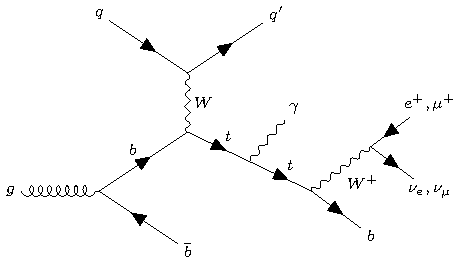
\includegraphics[width=0.9\textwidth]{Plots/s4_feyn_nom.pdf}
    \caption{Feynman diagram of the $tq\gamma$ process in the Standard Model.}
    \label{fig:feyn_tqGamma}
\end{figure}